\section{SMAWK}
\label{SMAWK}

%----------------------------------------------------------------------------------------

Nesta seção discutiremos o algoritmo SMAWK. Ele é conhecido pela sua aplicação no problema de encontrar o vértice mais distante de cada vértice num poígono convexo em tempo linear~\cite{Aggarwal:1987}. Ao final desta seção serão explicadas esta e outras aplicações deste algoritmo.  

Dada uma matriz $A \in \B{Q}^{n \times m}$, listamos os casos de uso deste algoritmo:
\begin{itemize}
    \item Se $A$ é totalmente monótona convexa ou côncava nas linhas podemos encontrar os índices de mínimos e máximos das linhas em tempo $\Cl{O}(n + m)$ e
    \item se $A$ é totalmente monótona convexa ou côncava nas colunas podemos encontrar os índices de mínimos e máximos das colunas em tempo $\Cl{O}(n + m)$.
\end{itemize}

Apresentaremos o caso onde $A$ é totalmente monótona convexa nas linhas e estamos interessados nos índices de mínimos. É fácil manipular o algoritmo para trabalhar com os outros casos.

%----------------------------------------------------------------------------------------

\subsection{Técnica Primordial} \label{SMAWK:primordial}
Para facilitar a compreensão do algoritmo SMAWK, iremos apresentar uma técnica parecida com a Divisão e Conquista apresentada na Seção~\ref{DivisaoEConquista} e mostrar uma otimização desta técnica que leva ao algoritmo SMAWK.

Dada uma matriz~$A \in \B{Q}^{n \times m}$ totalmente monótona convexa por linhas, queremos encontrar o menor índice de mínimo de cada uma das linhas de~$A$. Se para uma dada linha~$i$ onde~$i > 0$ e~$i < n$ conhecermos os índices~$l$ e~$r$ de mínimos das linhas~$i-1$ e~$i+1$, respectivamente, já que~$A$ tem os índices de mínimos das linhas crescente (por ser totalmente monótona) basta buscar o índice de mínimo da linha~$i$ no intervalo entre~$l$ e~$r$ (inclusive). Além disso, se~$i$ é a primeira linha da matriz podemos considerar~$l = 1$ ou se~$i$ é a última linha da matriz podemos considerar~$r = n$ sem perder a validade do fato de que basta buscar entre~$l$ e~$r$.  

Após realizar as observações acima note que, já que~$A$ é totalmente monótona, remover qualquer linha de~$A$ mantém a total monotonicidade e não altera o índice de mínimo de outra linha. Com esta observação, concluímos que podemos remover todas as linhas pares da matriz, resolver o problema recursivamente para a matriz resultante e utilizar este resultado para calcular os índices de interesse para as linhas pares da matriz. Vamos provar que encontrar estes índices de mínimos custa tempo~$\Cl{O}(m)$. 

Definimos a sequência~$t$ de forma que a~$i$-ésima linha ímpar de~$A$ busca seu máximo entre as colunas~$t_{i-1}$ e $t_{i}$, inclusive. Sabemos que~$0 = t_0 \leq t_1 \leq t_2 \leq \dots \leq t_{\floor{n/2}} \leq n$. Podemos escrever o tempo gasto por todas as buscas de mínimo como~$\sum \limits_{i=1}^{\floor{n/2}} t_i - t_{i-1} + 1 = \Cl{O}(n+m)$, ou seja, o trabalho feito para encontrar os mínimos das colunas ímpares dados os mínimos das colunas pares custa tempo~$\Cl{O}(n+m)$.

Agora, com uma análise similar à realizada para a técnica da Divisão e Conquista é fácil concluir que uma implementação desta técnica que consiga remover as linhas pares da matriz (e adicionar elas de volta) em tempo~$\Cl{O}(1)$ resolve o problema em tempo~$\Cl{O}((n+m)\lg(n))$, assim como a técnica da divisão e conquista.

%----------------------------------------------------------------------------------------

\subsection{Reduce} \label{SMAWK:reduce}
Queremos agilizar a técnica apresentada acima. Para isso, vamos adicionar uma nova hipótese. Vamos supor que a matriz~$A$ é quadrada, ou seja,~$n = m$. Lembre que a cada passo, removemos as~$\floor{n/2}$ linhas pares da matriz gerando uma nova matriz $A'$, resolvemos o problema recursivamente para~$A'$ e usamos a solução de~$A'$ para resolver para as linhas restantes de~$A$. O problema é que quando removemos linhas da nossa~$A$, ela deixa de ser quadrada e passa a ser uma matriz com mais colunas do que linhas, isto é,~$m \geq n$. Chamamos de ótimas as células da matriz que são mínimo de alguma linha e as colunas que contém o índice de mínimo de pelo menos uma linha. Note que uma matriz contém no máximo~$n$ colunas ótimas, pois cada linha faz com que exatamente uma célula seja ótima. Queremos remover colunas não ótimas de uma matriz~$A$ com mais colunas do que linhas fazendo com que~$A$ se torne quadrada.  

Vamos desenvolver o algoritmo \textsc{Reduce} a partir de um índice de linha~$k$ e de algumas invariantes: 
\begin{enumerate}
    \item Vale~$1 \leq k \leq n$, \label{invar:Reduce0}
    \item apenas colunas não ótimas foram removidas da matriz e \label{invar:Reduce1}
    \item toda célula em uma coluna de índice menor ou igual a~$k$ que possua índice de linha menor do que índice de coluna é não ótima. A Figura~\ref{figure:Reduce1} representa, em azul, a célula de índice~$k,k$ e, em preto, as células que, segundo esta invariante, são não ótimas. \label{invar:Reduce2}
\end{enumerate}

\begin{figure}[h]
    \centering
    % === Based On ===
% Geometric representation of the sum 1/4 + 1/16 + 1/64 + 1/256 + ...
% Author: Jimi Oke
% ================

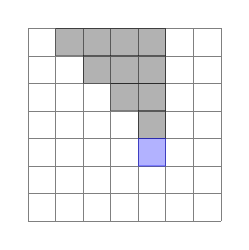
\begin{tikzpicture}[scale=.35]\footnotesize
 \pgfmathsetmacro{\xone}{0}
 \pgfmathsetmacro{\xtwo}{7}
 \pgfmathsetmacro{\yone}{0}
 \pgfmathsetmacro{\ytwo}{7}

\begin{scope}<+->;
% grid
  \draw[step=1cm,gray,very thin] (\xone,\yone) grid (\xtwo,\ytwo);
\end{scope}

% function
\begin{scope}[thin,black,opacity=.3]
  \filldraw (1,7) rectangle (5,6);
  \filldraw (2,6) rectangle (5,5);
  \filldraw (3,5) rectangle (5,4);
  \filldraw (4,4) rectangle (5,3);
  \filldraw[blue] (4,3) rectangle (5,2);
\end{scope}

\end{tikzpicture}

    \caption{Invariante~\ref{invar:Reduce2} do \textsc{Reduce}.} \label{figure:Reduce1}
\end{figure}

Vamos comparar~$A[k][k]$ com~$A[k][k+1]$ e considerar dois casos. Em cada um dos casos, concluiremos que algumas células da matriz $A$ são não ótimas. A Figura~\ref{figure:Reduce2} mostra, hachuradas em vermelho, as células que são descobertas não ótimas quando~$A[k][k] > A[k][k+1]$ e, com linhas verticais verdes, as células que são descobertas não ótimas quando~$A[k][k] \leq A[k][k+1]$. Vamos provar estas implicações.

\begin{figure}[h]
    \centering
    % === Based On ===
% Geometric representation of the sum 1/4 + 1/16 + 1/64 + 1/256 + ...
% Author: Jimi Oke
% ================

\begin{tikzpicture}[scale=.35]\footnotesize
 \pgfmathsetmacro{\xone}{0}
 \pgfmathsetmacro{\xtwo}{9}
 \pgfmathsetmacro{\yone}{0}
 \pgfmathsetmacro{\ytwo}{7}

\begin{scope}<+->;
% grid
  \draw[step=1cm,gray,very thin] (\xone,\yone) grid (\xtwo,\ytwo);
\end{scope}

% function
\begin{scope}[pattern=crosshatch dots,thin,pattern color=black,opacity=.3]
  \filldraw (1,7) rectangle (5,6);
  \filldraw (2,6) rectangle (5,5);
  \filldraw (3,5) rectangle (5,4);
  \filldraw (4,4) rectangle (5,3);
\end{scope}
\filldraw[blue,opacity=.3] (4,3) rectangle (5,2);
\filldraw[pattern=north west lines,pattern color=red] (4,3) rectangle (5,0);
\filldraw[pattern=vertical lines,pattern color=green] (5,7) rectangle (6,2);

\end{tikzpicture}

    \caption{Casos do \textsc{Reduce}.} \label{figure:Reduce2}
\end{figure}

Se~$A[k][k] > A[k][k+1]$, as entradas com índice de linha maior ou igual a~$k$ na coluna~$k$ são não ótimos. Primeiramente, a célula~$(k,k)$ é não ótima como consequência direta da desigualdade. Agora, suponha que existe alguma linha~$i>k$ tal que~$A[i][k] \leq A[i][k+1]$. Pela total monotonicidade convexa por linhas de $A$, isso implica em~$A[k][k] \leq A[k][k+1]$, um absurdo.  

Se~$A[k][k] \leq A[k][k+1]$, as células da coluna~$k+1$ com índices de linha menores ou iguals a~$k$ são não ótimas. A célula~$(k,k+1)$ é não ótima pela desigualdade apresentada. Supojnha que existe alguma linha~$i<k$ tal que~$A[i][k] > A[i][k+1]$. Pela contrapositiva da total monotonicidade, temos~$A[k][k] > A[k][k+1]$, um absurdo.  

Com estas observações estamos prontos para deduzir um algoritmo que elimina exatamente~$m-n$ colunas de~$A$. 

\newcommand{\Reduce}{\textsc{Reduce}}
\begin{algorithm}[H]
\caption{Algoritmo $\Reduce$}
\label{SMAWK:algo:Reduce}
\begin{algorithmic}[1]
\Function{\Reduce}{A}
    \State $k \rec 1$
    \While{$A$ tem mais linhas do que colunas}
        \If{$A[k][k] > A[k][k+1]$}
            \State Remove a coluna~$k$
            \State $k \rec \max(1,k-1)$
        \Else
            \If{$k = n$}
                \State Remove a coluna~$k+1$
            \Else
                \State $k \rec k+1$
            \EndIf
        \EndIf
    \EndWhile
    \State \Return $A$
\EndFunction
\end{algorithmic}
\end{algorithm}

É fácil ver que as invariantes são válidas neste algoritmo. Olhamos para o primeiro passo,~$k = 1$, nenhuma coluna foi removida ainda e não há elementos com índices de linha e coluna menores do que $k$, logo, as Invariantes~\ref{invar:Reduce0},~\ref{invar:Reduce1} e~\ref{invar:Reduce2} valem. Em todo passo do loop,~$A[k][k+1]$ existe, pois~$k \leq n$ e~$n \leq m$. Consideramos o caso onde~$A[k][k] > A[k][k+1]$, a Invariante~\ref{invar:Reduce0} sempre se mantém trivialmente, já provamos que a coluna~$k$ é não ótima neste caso, portanto, a Invariante~\ref{invar:Reduce1} se mantém mesmo após a remoção da coluna~$k$. Agora, se~$k=1$, vale a~\ref{invar:Reduce2} por vacuidade e, no caso contrário, já que a~$k$ decresce, a Invariante~\ref{invar:Reduce2} também se mantém. 

Em outro caso, valem~$A[k][k] \leq A[k][k+1]$ e $k = n$. Foi provado que os elemntos de linhas menores ou iguals a~$k$ na coluna coluna~$k+1$ são não ótimos, porém, isto representa toda a coluna~$k+1$, assim, remover ela mantém a Invariante~\ref{invar:Reduce1}. As outras duas invariantes se mantém trivialmente. Agora, falta considerar o caso onde~$A[k][k] \leq A[k][k+1]$ e $k < n$. Neste caso, foi provado, novamente, que as células com índices menores ou iguais a~$k$ na coluna~$k+1$ são inválidos. Estes são exatemente os elementos com índices de linhas menores do que índices de colunas na coluna~$k+1$, o que faz com que a Invariante~\ref{invar:Reduce2} se mantenha ao incrementarmos o valor de~$k$. As outras duas invariantes se mantém trivialmente neste caso.

Além disso, o algoritmo, a cada passo, incrementa~$k$ ou remove uma coluna de~$A$. Sabemos que~$k$ nunca passa de~$n$ e, já que a matriz tem~$m$ colunas, não podemos remover mais do que~$m$ colunas. Supondo que a cada remoção de coluna~$k$ seja decrementado, chegamos a uma quantidade máxima de~$2m + n$ passos. Supondo que as remoções sejam feitas em tempo constante, o tempo de cada passo é constante, portanto, atingimos uma complexidade de~$\Cl{O}(m)$ operações no algoritmo $\Reduce$, já que $n \leq m$.

%----------------------------------------------------------------------------------------

\subsection{SMAWK}
\newcommand{\SMAWK}{\textsc{SMAWK}}

Recebemos uma matriz~$A \in \B{Q}^{n \times m}$ totalmente monótona convexa por linhas. Primeiramente, vamos transformar a matriz $A$ em uma matriz quadrada. Se~$A$ tem mais colunas do que linhas, basta aplicar o algorimto~$\Reduce$ em~$A$ para fazer com que ela fique quadrada e tenha os mesmos índices de mínimos. Se~$A$ tem mais linhas do que colunas, basta adicionar colunas sem que os mínimos ou a total monotonicidade sejam prejudicados, para isso, adicionamos, ao final da matriz, colunas~$n-m$ com entradas infinitas. 

Agora estamos prontos para descrever e aplicar o algoritmo~$\SMAWK$ na matriz modificada. Vamos misturar as ideias apresentadas da técnica primordial, apresentada na Subseção~\ref{SMAWK:primordial}, e do~$\Reduce$, apresentado na Subseção~\ref{SMAWK:reduce}. Em cada passo, removemos as linhas pares da matriz, aplicamos o algoritmo $\Reduce$ para manter esta nova matriz quadrada e resolvemos o problema recursivamente para a nova matriz. Com a solução desta instância, descobrimos os resultados para as linhas restantes da matriz original. O Algoritmo~\ref{SMAWK:algo:SMAWK} descreve este processo.

\begin{algorithm}[H]
\caption{Algoritmo $\SMAWK$}
\label{SMAWK:algo:SMAWK}
\begin{algorithmic}[1]
\Function{\SMAWK}{A}
    \If{$A$ tem uma linha}
        \State $A$ é uma matriz~$1 \times 1$ e a resposta é trivial
    \Else
        \State Retiramos as linhas pares de~$A$ gerando~$A'$
        \State $A'' \rec \Reduce(A')$
        \State $\SMAWK(A'')$
        \For{$i$ linha ímpar de $A$}
            \State $l \rec 1$ e $r \rec m$
            \If{$i > 1$}
                \State $l \rec$ índice de mínimo da linha~$i - 1$
            \EndIf
            \If{$i < n$}
                \State $r \rec$ índice de mínimo da linha~$i + 1$
            \EndIf
            \State Busca o índice de mínimo da linha~$i$ entre~$l$ e~$r$, inclusive
        \EndFor
    \EndIf
\EndFunction
\end{algorithmic}
\end{algorithm}

%----------------------------------------------------------------------------------------

\subsection{Análise}
O tempo gasto pelo algoritmo~$\SMAWK$ depende apenas da dimensão~$n$ da matriz recebida. Escrevemos~$T(n)$ a recorrência que define o tempo gasto pelo algoritmo para todo~$n \geq 1$. Sabemos que~$T(1) = \Cl{O}(1)$. Com~$n > 1$, a retirada de linhas pares será implementada em tempo constante, o algoritmo~$\Reduce$ é, então, aplicado a uma matriz com~$\floor{n/2}$ linhas e~$n$ colunas, gastando tempo~$\Cl{O}(n)$ e depois os máximos das lunhas ímpares de~$A$ são achados à partir das linhas pares de~$A$ na forma descrita na Subseção~\ref{SMAWK:primordial}, o que custa tempo~$\Cl{O}(n)$. Assim, para todo~$n>1$,~$T(n) = \Cl{O}(n) + T(\floor{n/2})$, o que nos leva a~$T(n) = \Cl{O}(n)$.

Se a matriz recebida tiver menos colunas do que linhas, a transformação inicial custa tempo~$\Cl{O}(n)$, no outro caso, custa tempo~$\Cl{O}(m)$, onde~$m$ é a quantidade de colunas. Assim, podemos escrever a complexidade no caso geral como~$\Cl{O}(n+m)$.

%----------------------------------------------------------------------------------------

\subsection{Implementação}
Queremos encontrar uma maneira eficiente de remover as linhas pares da matriz, mas não podemos gerar explicitamente uma nova matriz. Queremos representar, a cada passo, todas as linhas que podem ser visitadas. Se~$k$ é um inteiro não negativo arbitrário, as linhas da matriz são da forma~$1 + k$, as linhas visitáveis após a retirada de todas as pares são da forma~$1 + 2k$, as visitáveis depois de duas remoções são da forma~$1 + 4k$ e assim por diante, ou seja, depois de~$t$ remoções de linhas pares, podemos visitar as linhas da forma~$1 + 2^tk$. Assim, basta guardar o inteiro~$p = 2^t$ para representar todas as linhas que podem ser visitadas pelo algoritmo em um dado passo. Remover todas as linhas pares é dobrar o valor de~$p$.  

Agora, precisamos representar as colunas visitáveis em~$A$. Já que não há uma regra fixa para a remoção de colunas, precisamos de alguma estrutura de dados que nos permita iterar pelos seus valores em ordem e remover um valor eficientemente sempre que visitado. Guardaremos uma lista duplamente ligada com todos os índices de colunas válidos, já que iteramos pelas colunas e, quando removemos uma coluna, ela é sempre vizinha da atual ou a atual, as remoções são feitas em $\Cl{O}(1)$. Após resolver o problema recursivamente, precisamos recuperar as informações desta lista ligada ao início da iteração para podermos descobrir os valores de mínimo nas linhas ímpares daquela matriz, para isso, basta, ao começo de cada passo, criar uma cópia da lista ligada original, o que é feito em~$\Cl{O}(n)$ e não afeta a análise do tempo do algoritmo.

No início do algoritmo, precisamos gerar a lista ligada original e, caso haja mais colunas do que linhas, aplicar uma vez o algoritmo~$\Reduce$. Caso a quantidade de linhas seja maior do que a de colunas, precisamos criar uma nova matriz com colunas a mais do que a original. Já que nossas matrizes são representadas por funções, suponha que o algoritmo recebe uma função~$f$ e dois inteiros~$n$, quantidade de linhas, e~$m$, quantidade de colunas. Podemos criar uma função~$h$ definida, para todo~$1 \leq i,j \leq n$ como~$f(i,j)$ se~$j \leq m$ e~$+\infty$ caso contrário e substituir~$f$ por esta no restante do algoritmo.

A implementação em C++ do algoritmo apresentado, levando em conta as considerações acima, pode ser encontrada em \texttt{implementacao/SMAWK.cpp}.

%----------------------------------------------------------------------------------------

%\subsection{Aplicação em programação dinâmica} // comparar com DivConq
%\subsection{Aplicação em geometria}            // all vertices furthest convex poly
